\documentclass{jarticle}
\usepackage[top=20truemm,bottom=15truemm,left=20truemm,right=20truemm]{geometry}
\usepackage{jlisting, listings, here}
\usepackage[dvipdfmx]{graphicx}
\makeatletter
\def\maketitle{%
\null
\thispagestyle{empty}%
\vfill
\begin{center}\leavevmode
\normalfont
{\LARGE \@title\par}%
\vskip 1cm
{\Large \@author\par}%
\vskip 1cm
{\Large \@date\par}%
\end{center}%
\vfill
\null
\@thanks%\vfil\null
\cleardoublepage
}
\makeatother
\lstset{language=c,
basicstyle=\ttfamily\scriptsize,
commentstyle=\textit,
classoffset=1,
keywordstyle=\bfseries,
frame=tRBl,
framesep=5pt,
showstringspaces=false,
stepnumber=1,
numberstyle=\tiny,
tabsize=2,
numbers = left,
stepnumber=1
}
\title{ソフトウェア演習V 課題3(再提出)}
\author{15122013 尾持涼介}
\date{提出日:2018年2月9日}

\begin{document}
\maketitle

\section{作成したプログラムの設計情報}
\subsection{全体構成}
各ファイルで記述した関数は以下の通りである。
\begin{itemize}
  \item main.c
  \begin{itemize}
    \item main関数
    \item void error(char *mes)
  \end{itemize}
  \item scan.c
  \begin{itemize}
    \item int init\_scan(char *filename)
    \item int keyword\_search(char *string)
    \item int scan()
    \item int get\_linenum()
    \item void end\_scan()
  \end{itemize}
  \item prettyprinter.c
  \begin{itemize}
    \item int parse\_program()
    \item int block()
    \item int var\_decl()
    \item int var\_names()
    \item int type()
    \item int ar\_type()
    \item int sub\_decl()
    \item int form\_para()
    \item int fukugou()
    \item int statement()
    \item int bunki()
    \item int kurikaeshi()
    \item int call\_st()
    \item int exp\_narabi()
    \item int dainyu()
    \item int var()
    \item int shiki()
    \item int simple()
    \item int kou()
    \item int inshi()
    \item int input\_st()
    \item int output\_st()
    \item int shitei()
  \end{itemize}
  \item crossreferencer.c
  \begin{itemize}
    \item void init\_idtab()
    \item struct ID *search\_globalidtab(char *np)
    \item struct ID *search\_localidtab(char *np)
    \item int globalid\_def()
    \item int procedure\_def()
    \item int globalid\_ref(char *np)
    \item int localid\_def()
    \item int localid\_ref(char *np)
    \item int type\_mem(struct ID *p)
    \item void printtab()
    \item void inorder(struct ID *p)
    \item void joint\_localtoglobal()
    \item void release\_idtab()
  \end{itemize}
\end{itemize}
次に、各関数の呼び出し関係、データ参照関係について述べる。
\begin{itemize}
  \item main.c
  \begin{itemize}
    \item main関数内
    \begin{itemize}
      \item init\_scan()関数を呼び出し
      \item scan()関数を呼び出し
      \item parse\_program()関数を呼び出し
      \item printtab()関数を呼び出し
      \item end\_scan()関数を呼び出し
    \end{itemize}
    \item error関数内
    \begin{itemize}
      \item get\_linenum()関数を参照
    \end{itemize}
  \end{itemize}
  \item scan.c
  \begin{itemize}
    \item scan()関数内
    \begin{itemize}
      \item keyword\_search()関数を呼び出し
      \item error()関数を呼び出し
    \end{itemize}
  \end{itemize}
  \item prettyprinter.c
  \begin{itemize}
    \item parse\_program()関数内
    \begin{itemize}
      \item error()関数を呼び出し
      \item scan()関数を呼び出し
      \item block()関数を呼び出し
    \end{itemize}
    \item block()関数内
    \begin{itemize}
      \item var\_decl()関数を呼び出し
      \item sub\_decl()関数を呼び出し
      \item fukugou()関数を呼び出し
    \end{itemize}
    \item var\_decl()関数内
    \begin{itemize}
      \item scan()関数を呼び出し
      \item var\_names()関数を呼び出し
      \item  error()関数を呼び出し
      \item type()関数を呼び出し
      \item globalid\_def()関数を呼び出し
      \item localid\_def()関数を呼び出し
    \end{itemize}
    \item var\_names()関数内
    \begin{itemize}
      \item error()関数を呼び出し
      \item scan()関数を呼び出し
      \item ar\_types()関数を呼び出し
    \end{itemize}
    \item type()関数内
    \begin{itemize}
      \item scan()関数を呼び出し
      \item ar\_type()関数を呼び出し
      \item error()関数を呼び出し
    \end{itemize}
    \item ar\_types()関数内
    \begin{itemize}
      \item scan()関数を呼び出し
      \item error()関数を呼び出し
    \end{itemize}
    \item sub\_decl()関数内
    \begin{itemize}
      \item scan()関数を呼び出し
      \item error()関数を呼び出し
      \item procedure\_def()関数を呼び出し
      \item form\_para()関数を呼び出し
      \item var\_decl()関数を呼び出し
      \item fukugou()関数を呼び出し
      \item joint\_localtoglobal()関数の呼び出し
    \end{itemize}
    \item form\_para()関数内
    \begin{itemize}
      \item scan()関数を呼び出し
      \item var\_names()関数を呼び出し
      \item error()関数を呼び出し
      \item type()関数を呼び出し
      \item localid\_def()関数を呼び出し
    \end{itemize}
    \item fukugou()関数内
    \begin{itemize}
      \item error()関数を呼び出し
      \item scan()関数を呼び出し
      \item statement()関数を呼び出し
    \end{itemize}
    \item statemen()関数内
    \begin{itemize}
      \item dainyu()関数を呼び出し
      \item bunki()関数を呼び出し
      \item kurikaeshi()関数を呼び出し
      \item scan()関数を呼び出し
      \item call\_st()関数を呼び出し
      \item input\_st()関数を呼び出し
      \item output\_st()関数を呼び出し
      \item fukugou()関数を呼び出し
    \end{itemize}
    \item bunki()関数内
    \begin{itemize}
      \item scan()関数を呼び出し
      \item shiki()関数を呼び出し
      \item error()関数を呼び出し
      \item statement()関数を呼び出し
    \end{itemize}
    \item kurikaeshi()関数内
    \begin{itemize}
      \item scan()関数を呼び出し
      \item shiki()関数を呼び出し
      \item error()関数を呼び出し
      \item statement()関数を呼び出し
    \end{itemize}
    \item call\_st()関数内
    \begin{itemize}
      \item scan()関数を呼び出し
      \item error()関数を呼び出し
      \item globalid\_ref()関数を呼び出し
      \item localid\_ref()関数を呼び出し
      \item exp\_narabi()関数を呼び出し
    \end{itemize}
    \item exp\_narabi()関数内
    \begin{itemize}
      \item shiki()関数を呼び出し
      \item error()関数を呼び出し
    \end{itemize}
    \item dainyu()関数内
    \begin{itemize}
      \item var()関数を呼び出し
      \item error()関数を呼び出し
      \item scan()関数を呼び出し
      \item shiki()関数を呼び出し
    \end{itemize}
    \item var()関数内
    \begin{itemize}
      \item error()関数を呼び出し
      \item globalid\_ref()関数を呼び出し
      \item localid\_ref()関数を呼び出し
      \item scan()関数を呼び出し
      \item shiki()関数を呼び出し
    \end{itemize}
    \item shiki()関数内
    \begin{itemize}
      \item simple()関数を呼び出し
      \item scan()関数を呼び出し
    \end{itemize}
    \item simple()関数内
    \begin{itemize}
      \item kou()関数を呼び出し
      \item error()関数を呼び出し
      \item scan()関数を呼び出し
      \item error()関数を呼び出し
    \end{itemize}
    \item kou()関数内
    \begin{itemize}
      \item inshi()関数を呼び出し
      \item error()関数を呼び出し
      \item scan()関数を呼び出し
    \end{itemize}
    \item inshi()関数内
    \begin{itemize}
      \item var()関数を呼び出し
      \item scan()関数を呼び出し
      \item shiki()関数を呼び出し
      \item error()関数を呼び出し
      \item inshi()関数を呼び出し
    \end{itemize}
    \item input\_st()関数内
    \begin{itemize}
      \item scan()関数を呼び出し
      \item var()関数を呼び出し
      \item error()関数を呼び出し
    \end{itemize}
    \item output\_st()関数内
    \begin{itemize}
      \item scan()関数を呼び出し
      \item shitei()関数を呼び出し
      \item error()関数を呼び出し
    \end{itemize}
    \item shitei()関数内
    \begin{itemize}
      \item scan()関数を呼び出し
      \item shiki()関数を呼び出し
      \item error()関数を呼び出し
    \end{itemize}
  \end{itemize}
  \item crossreferencer.c内
  \begin{itemize}
    \item globalid\_def()関数内
    \begin{itemize}
      \item error()関数を呼び出し
      \item get\_linenum()関数を呼び出し
      \item type\_mem()関数を呼び出し
    \end{itemize}
    \item procedure\_def()関数内
    \begin{itemize}
      \item error()関数を呼び出し
      \item get\_linenum()関数を呼び出し
      \item type\_mem()関数を呼び出し
    \end{itemize}
    \item globalid\_ref()関数内
    \begin{itemize}
      \item search\_globalidtab()関数を呼び出し
      \item get\_linenum()関数を呼び出し
      \item error()関数を呼び出し
    \end{itemize}
    \item lobalid\_def()関数内
    \begin{itemize}
      \item error()関数を呼び出し
      \item type\_mem()関数を呼び出し
      \item get\_linenum()関数を呼び出し
    \end{itemize}
    \item localid\_ref()関数内
    \begin{itemize}
      \item search\_localidtab()関数を呼び出し
      \item error()関数を呼び出し
      \item get\_linenum()関数を呼び出し
      \item search\_globalidtab()関数を呼び出し
    \end{itemize}
    \item type\_mem()関数内
    \begin{itemize}
      \item error()関数を呼び出し
    \end{itemize}
    \item printtab()関数内
    \begin{itemize}
      \item error関数を呼び出し
      \item inorder関数を呼び出し
    \end{itemize}
    \item inorder関数内
    \begin{itemize}
      \item inorder関数を呼び出し(再帰呼出し)
    \end{itemize}
    \item joint\_localtoglobal関数内
    \begin{itemize}
      \item error()関数を呼び出し
    \end{itemize}
    \item release\_idtab()関数内
    \begin{itemize}
      \item release\_idtab()関数を呼び出し(再帰呼出し)
      \item init\_idtab()関数を呼び出し
    \end{itemize}
  \end{itemize}
\end{itemize}
\subsection{各モジュールごとの構成}
大域変数(手続き名も含む)、と局所変数(仮引数として定義されたものも含む)を二分探索木で記憶するために、以下の図\ref{code:list}のような
構造体を定義した。
\begin{figure}[H]
\begin{center}
\begin{lstlisting}
struct ID {
char *name;
char *procname;
struct TYPE *itp;
int ispara;
int deflinenum;
struct LINE *irefp;
struct ID *left, *right;
} ;
\end{lstlisting}
\caption{大域変数、局所変数を記憶するための二分探索木の構造体}
\label{code:list}
\end{center}
\end{figure}
なお、ここで、nameはその変数の名前、procnameはその変数が局所変数か仮引数であるときにその変数が定義されている関数名、itpは
その変数の型、isparaはその変数が仮引数かそれ以外か(仮引数なら1、それ以外なら0)、deflinenumはその変数が定義された行、irefpはその変数が使用された行、
leftとrightはそれぞれ、左部分木、右部分木を指すポインタである。このように定義することにより、inorder関数で辞書順に出力することができる。「struct
TYPE」と「struct LINE」はそれぞれ変数の型、出現した行を記憶するために以下の図\ref{code:type}、\ref{code:line}のように定義された構造体である。
\begin{figure}[H]
\begin{center}
\begin{lstlisting}
struct TYPE{
int ttype;
int arraysize;
struct TYPE *etp;
struct TYPE *paratp;
};
\end{lstlisting}
\caption{型を記憶するための構造体}
\label{code:type}
\end{center}
\end{figure}
\begin{figure}[H]
\begin{center}
\begin{lstlisting}
struct LINE{
int reflinenum;
struct LINE *nextlinep;
};
\end{lstlisting}
\caption{出現した行を記憶するための構造体}
\label{code:line}
\end{center}
\end{figure}
ここで図\ref{code:type}においてttypeはその変数の型を表す整数、arraysizeはその変数が配列型であった場合の要素数、
etpはその変数が配列型であった場合の要素の型、paratpはその変数がprocedureつまり手続き名であったときに仮引数の型を指すポインタである。
すなわち、副プログラムの仮引数を格納する際には線形リストとして用いている。
図\ref{code:line}においてreflinenumはその行数、nextlinepは線形リストの次の要素を指す
ポインタである。

また、変数宣言部において宣言される変数名のうち、コンマによって連続して宣言された同じ型の変数名を記憶するために
以下の図\ref{code:name}のような構造体を定義して、線形リストとして用いた。
\begin{figure}
\begin{center}
\begin{lstlisting}
struct NAME{
char *name;
struct NAME *next;
};
\end{lstlisting}
\caption{変数名を記憶する構造体}
\label{code:name}
\end{center}
\end{figure}

なお、型を表す整数は次の図\ref{code:kata}のよう定義し、型名を格納する配列をcrossreferencer.c内で図\ref{code:katahairetu}のように定義している。
\begin{figure}[H]
\begin{center}
\begin{lstlisting}
#define TPINT 1 /* integer */
#define TPCHAR 2 /* char */
#define TPBOOL 3 /* boolean */
#define TPARRAY 4 /* array */
#define TPPROC 5 /* procedure */
\end{lstlisting}
\caption{型を表す整数}
\label{code:kata}
\end{center}
\end{figure}
\begin{figure}[H]
\begin{center}
\begin{lstlisting}
char *typename[NUMOFTYPE + 1] = {
"",
"integer", "char", "boolean", "array", "procedure"
};
\end{lstlisting}
\caption{型名を格納する配列}
\label{code:katahairetu}
\end{center}
\end{figure}
NUMMOFTYPEはこの配列に格納した型名の数であり、5とヘッダファイル内で定義されている。

そして、局所変数用二分探索木はその副プログラム宣言が終了するときに大域変数用二分探索木に追加して、最後にまとめて
出力している。そのことにより、辞書順に出力される。

名前は全文字列が一致している場合にのみ同一の名前とした。

次に使用した大域変数とその意味について述べる。

\begin{itemize}
  \item main.c内
  \begin{itemize}
    \item struct KEY key[KEYWORDSIZE] :予約語(キーワード)が格納されている。
    \item char *tokenstr[NUMOFTOKEN+1] :各トークン名が格納されている。
    \item int token:読み込んだトークンのトークン番号が格納されている。
  \end{itemize}
  \item scan.c内
  \begin{itemize}
    \item 課題2のレポートで説明済み。
  \end{itemize}
  \item prettyprinter.c内
  \begin{itemize}
    \item int arrayflag:その前に出てきた変数が配列型かどうかを表す変数(1なら配列型、0なら標準型)
    \item int arraynum:配列型の要素数を格納する変数
    \item int typenum:宣言された変数の型を表す整数を格納する。
    \item int paraflag:今調べている変数が仮引数かどうかを記憶する変数(1なら仮引数、0ならその他)。
    \item int gorl:調べている変数が大域変数か局所変数かを記憶する変数(1なら局所変数、0なら大域変数)。
    \item int arraytype:配列の要素の型を表す整数を格納する。
    \item int shikitype:「式」の型を表す整数を格納する。
    \item int shikiarraysize:「式」が配列型であるときに要素数を記憶する変数。
    \item int shikiarraytype:「式」が配列型であるときにその要素の型を記憶する変数。
    \item int vartype:「変数」の型を表す整数を格納する。
    \item int vararraysize:「変数」が配列型であるときに要素数を記憶する変数。
    \item int vararraytype:「変数」が配列型であるときにその要素の型を記憶する変数。
    \item int koutype:「項」の型を表す整数を格納する。
    \item int kouarraysize:「項」が配列型であるときに要素数を記憶する変数。
    \item int kouarraytype:「項」が配列型であるときにその要素の型を記憶する変数。
    \item int inshitype:「因子」の型を表す整数を格納する。
    \item int inshiarraysize:「因子」が配列型であるときに要素数を記憶する変数。
    \item int inshiarraytype:「因子」が配列型であるときにその要素の型を記憶する変数。
    \item int paranum:仮引数の個数を記憶する変数。
    \item int expnum:式の並びにおいて式の個数を記憶する変数。
    \item struct NAME *names:変数宣言部、仮引数部における変数名の並びを記憶する線形リストの先頭要素を指すポインタ。
    \item struct TYPE *paratype:仮引数の型を記憶する線形リストの先頭要素を指すポインタ。
    \item struct ID *searchp:局所変数・大域変数の二分探索木のうち、探索した変数名の要素を指すポインタ。
  \end{itemize}
  \item crossreferencer.c内
  \begin{itemize}
    \item struct ID *globalidroot:大域変数を格納する二分探索木の先頭要素を指すポインタ。
    \item struct ID *localidroot:局所変数を格納する二分探索木の先頭要素を指すポインタ。
    \item char *typename[NUMOFTYPE+1]:型名を格納した配列。
  \end{itemize}
\end{itemize}

次に各関数内で定義した変数とその意味について述べる

\begin{itemize}
  \item scan.c
  \begin{itemize}
    \item ikeyword\_search()関数内:課題1で記載済み
    \item scan()関数内
    \begin{itemize}
      \item int i:課題1で記載済み
    \end{itemize}
  \end{itemize}
  \item prettyprinter.c
  \begin{itemize}
    \item var\_names()内
    \begin{itemize}
      \item struct NAME *p:namesに追加する要素を指すポインタ。
      \item struct NAME *q:作成した要素をnamesに挿入するためにnamesをたどるポインタ。
      \item char *cp:線形リストに格納する変数名を格納するポインタ。
    \end{itemize}
    \item type()内
    \begin{itemize}
      \item int a:ar\_type()関数からの返り値を記憶する変数。
    \end{itemize}
    \item form\_para()関数内
    \begin{itemize}
      \item struct NAME *n:for文でnamesを辿るためのポインタ。
      \item struct TYPE *p:新たな仮引数の型情報を格納するポインタ。
      \item struct TYPE *q:pがさす要素をparatpにつなげるためのポインタ。
    \end{itemize}
    \item bunki()関数内
    \begin{itemize}
      \item int flag:課題2で記載済み。
    \end{itemize}
    \item kurikaeshi()関数内
    \begin{itemize}
      \item
      int
      flag:課題2で記載済み
    \end{itemize}
    \item call\_st()関数内
    \begin{itemize}
      \item struct TYPE *q:呼び出し文で呼び出された副プログラムの仮引数の型情報を記憶する構造体の先頭要素を指すポインタ。
    \end{itemize}
    \item exp\_narabi()関数内
    \begin{itemize}
      \item struct TYPE *p:式の型情報を記憶する構造体の先頭要素を指すポインタ。
    \end{itemize}
    \item dainyu()関数内
    \begin{itemize}
      \item int type1:左辺値の型を記憶する変数。
      \item int type2:代入する式の型を記憶する変数。
    \end{itemize}
    \item var()関数内
    \begin{itemize}
      \item int arraytype:変数名が配列型の場合その要素の型を記憶する変数。
    \end{itemize}
    \item shiki()関数内
    \begin{itemize}
      \item int type1, type2:それぞれの直前で出現した単純式の型を記憶する変数。
      \item int
      arraysize1、arraysize2:それぞれの直前に出現した単純式が配列型だった場合にその要素数を記憶する変数。
      \item int
      arraytype1、arraytype2:それぞれの直前に出現した単純式が配列型だった場合にその要素の型を記憶する変数。
    \end{itemize}
    \item simple()関数内
    \begin{itemize}
      \item int flag:最初の項の前に+か-があるかどうかを示す変数(0ならない、1ならある)。
      \item int type1, type2:それぞれの直前に出現した項の型を記憶する変数。
      \item int kahou:加法演算子を記憶する変数。
    \end{itemize}
    \begin{itemize}
      \item int type1, type2:それぞれの直前に出現した因子の型を記憶する変数。
      \item int jouhou:情報演算子を記憶する変数。
    \end{itemize}
    \item inshi()関数内
    \begin{itemize}
      \item int type1:因子の最初に標準型がある場合にその型を記憶する変数。
    \end{itemize}
  \end{itemize}
  \item crossreferencer.c内
  \begin{itemize}
    \item search\_globalidtab()関数内
    \begin{itemize}
      \item struct ID *p:for文による探索のためにglobalrootを辿るポインタ。
    \end{itemize}
    \item search\_localidtab()関数内
    \begin{itemize}
      \item struct ID *p:for文による探索のためにlocalrootを辿るポインタ。
    \end{itemize}
    \item globalid\_def()関数内
    \begin{itemize}
      \item struct ID *new;新しくglobalrootにつなげる要素を指すポインタ。
      \item struct ID *p;globalidrootを辿るポインタ。
      \item struct NAME *np:namesのうちglobalidrootに登録する要素を指すポインタ。
      \item struct NAME *nq:for文でnamesを辿るためのポインタ。
    \end{itemize}
    \item procedure\_def()関数内
    \begin{itemize}
      \item struct ID *new;新しくglobalrootにつなげる要素を指すポインタ。
      \item struct ID *p;globalidrootを辿るポインタ。
      \item char *cp:新しく加える手続き名を指すポインタ。
    \end{itemize}
    \item globalid\_ref()関数内
    \begin{itemize}
      \item struct ID *p:探索した要素を指すポインタ。
      \item struct LINE *next:新たに出現した行を格納すべき要素を指すポインタ。
      \item struct LINE *prev:新たに出現した行を格納すべき要素の1つ前を指すポインタ。
      \item struct LINE *m:新たに付け加える行番号を格納した要素を指すポインタ。
    \end{itemize}
    \item localid\_def()関数内
    \begin{itemize}
      \item struct ID *new;新しくlocalrootにつなげる要素を指すポインタ。
      \item struct ID *p;locaidrootを辿るポインタ。
      \item struct NAME *np:namesのうちglobalidrootに登録する要素を指すポインタ。
      \item struct NAME *nq:for文でnamesを辿るためのポインタ。
      \item char *cp:その局所変数が定義されている手続き名を格納するポインタ。
    \end{itemize}
    \item localid\_ref()関数内
    \begin{itemize}
      \item struct ID *p:探索した要素を指すポインタ。
      \item struct LINE *next:新たに出現した行を格納すべき要素を指すポインタ。
      \item struct LINE *prev:新たに出現した行を格納すべき要素の1つ前を指すポインタ。
      \item struct LINE *m:新たに付け加える行番号を格納した要素を指すポインタ。
    \end{itemize}
    \item type\_mem()関数内
    \begin{itemize}
      \item struct TYPE *q:新しく追加する型情報を格納した要素を指すポインタ。
      \item struct TYPE *r:新しく追加する型が配列型の時の要素の型情報を格納するポインタ。
      \item struct TYPE *pt:仮引数の型情報を記憶するときにparatypeを辿るポインタ。
    \end{itemize}
    \item printtab()関数内
    \begin{itemize}
      \item int i:ループ変数。
      \item space1:名前を出力してから型名を出力するまでどれだけ空白を開けるかを示す変数。
      \item space2:型名を出力したから定義された行番号を出力するまでどれだけ空白を開けるかを示す変数。
      \item char *cp:大域変数は変数名(手続き名)を、局所変数のときは変数名にコロンと手続き名を足したものを格納するポインタ。
      \item char ar[100]:配列型の要素数を文字列に変換したものを格納する配列。
    \end{itemize}
    \item inorder()関数内
    \begin{itemize}
      \item struct LINE *q:出現した行番号を出力するときに行情報のリストを辿るポインタ。
      \item int i:ループ変数。
      \item space1:名前を出力してから型名を出力するまでどれだけ空白を開けるかを示す変数。
      \item space2:型名を出力したから定義された行番号を出力するまでどれだけ空白を開けるかを示す変数。
      \item char *cp:大域変数は変数名(手続き名)を、局所変数のときは変数名にコロンと手続き名を足したものを格納するポインタ。
      \item char ar[100]:配列型の要素数を文字列に変換したものを格納する配列。
    \end{itemize}
    \item joint\_localtoglobal()関数内
    \begin{itemize}
      \item struct ID *x:globalrootにつなげた要素を指すポインタ
      \item struct ID **p:globalidrootを辿るためのポインタ。
      \item struct ID **q:localidrootを辿るためのポインタ
    \end{itemize}
  \end{itemize}
\end{itemize}
\subsection{各関数の外部(入出力)仕様}
ここでは、各関数の機能、引数と返り値等について説明する。
\subsubsection{main.c内で記述されている関数}
\begin{itemize}
  \item main関数
  \begin{description}
\item[引数]コマンドライン引数としてint ncとchar
*np[]を指定する。ncは指定された引数の個数を表し、npはプログラムを起動するときに指定する引数であり、本プログラムでは読み込むファイル名を指定する。
\item[返り値]プログラムが終了した際に0を返す。
\item[参照・変更する大域変数]token
\end{description}
\item void error(char *mes):課題2で記載済み
\end{itemize}
\subsubsection{scan.c内で記述されている関数}
\begin{itemize}
  \item int init\_scan(char *filename):課題1で記載済み
  \item int keyword\_search(char *string):課題1で記載済み
  \item int scan():課題2で記載済み
  \item int get\_linenum():課題1で記載済み
  \item void end\_scan():課題1で記載済み
\end{itemize}
\subsubsection{prettyprinter.c内で記述した関数}
なお、以下でNORMALとERRORはそれぞれprettyprinter.c内で0、1と定義されている。
\begin{itemize}
  \item int parse\_program()
  \begin{description}
\item[機能]プログラムを解析する関数
\item[引数]なし
\item[返り値]エラーがあればERRORを、なければNORMALを返す。
\item[参照・変更する大域変数]token
\end{description}
\item int block()
\begin{description}
\item[機能]ブロックを解析する関数
\item[引数]なし
\item[返り値]エラーがあればERRORを、なければNORMALを返す。
\item[参照する大域変数]token
\end{description}
\item int var\_decl
\begin{description}
\item[機能]変数宣言部を解析する関数
\item[引数]なし
\item[返り値]エラーがあればERRORを、なければNORMALを返す。
\item[変更する大域変数]token
\item[参照する大域変数]gorl、token
\end{description}
\item int var\_names()
\begin{description}
\item[機能]変数名の並びを解析する関数
\item[引数]なし
\item[返り値]エラーがあればERRORを、なければNORMALを返す。
\item[変更する大域変数]token, names
\item[参照する大域変数]string\_attr、token
\end{description}
\item int type()
\begin{description}
\item[機能]型を解析する関数
\item[引数]なし
\item[返り値]エラーがあればERRORを、なければNORMALを返す。
\item[参照・変更する大域変数]token
\end{description}
\item int ar\_type()
\begin{description}
\item[機能]配列型を解析する関数
\item[引数]なし
\item[返り値]エラーがあればERRORを、なければNORMALを返す。
\item[変更する大域変数]token、typenum、arraynum
\item[参照する大域変数]token、string\_attr、num\_attr
\end{description}
\item int sub\_decl()
\begin{description}
\item[機能]副プログラム宣言を解析する関数
\item[引数]なし
\item[返り値]エラーがあればERRORを、なければNORMALを返す。
\item[変更する大域変数]token、gorl、localidroot、procname
\item[参照する大域変数]token、string\_attr
\end{description}
\item int form\_para()
\begin{description}
\item[機能]仮引数部を解析する関数
\item[引数]なし
\item[返り値]エラーがあればERRORを、なければNORMALを返す。
\item[変更する大域変数]token、paratype、paraflag
\item[参照する大域変数]names、token、typenum
\end{description}
\item int fukugou()
\begin{description}
\item[機能]複合文を解析する関数
\item[引数]なし
\item[返り値]エラーがあればERRORを、なければNORMALを返す。
\item[参照・変更する大域変数]token
\end{description}
\item int statement()
\begin{description}
\item[機能]文を解析する関数
\item[引数]なし
\item[返り値]エラーがあればERRORを、なければNORMALを返す。
\item[参照・変更する大域変数]token
\end{description}
\item int bunki()
\begin{description}
\item[機能]分岐文を解析する関数
\item[引数]なし
\item[返り値]エラーがあればERRORを、なければNORMALを返す。
\item[参照・変更する大域変数]token、indentnum
\end{description}
\item int kurikaeshi()
\begin{description}
\item[機能]繰り返し文を解析する関数
\item[引数]なし
\item[返り値]エラーがあればERRORを、なければNORMALを返す。
\item[変更する大域変数]token、
\item[参照する大域変数]shikitype、token
\end{description}
\item int call\_st()
\begin{description}
\item[機能]手続き呼び出し文を解析する関数
\item[引数]なし
\item[返り値]エラーがあればERRORを、なければNORMALを返す。
\item[変更する大域変数]token、paranum、expnum
\item[参照する大域変数]gorl、token、string\_attr、procname、searchp、paranum、expnum
\end{description}
\item int exp\_narabi()
\begin{description}
\item[機能]式の並びを解析する関数
\item[引数]なし
\item[返り値]エラーがあればERRORを、なければNORMALを返す。
\item[変更する大域変数]token、expnum
\item[参照する大域変数]token、searchp、shikitype、
\end{description}
\item int dainyu()
\begin{description}
\item[機能]代入文を解析する関数
\item[引数]なし
\item[返り値]エラーがあればERRORを、なければNORMALを返す。
\item[変更する大域変数]token
\item[参照する大域変数]vartype、shikitype、token
\end{description}
\item int var()
\begin{description}
\item[機能]変数を解析する関数
\item[引数]なし
\item[返り値]エラーがあればERRORを、なければNORMALを返す。
\item[変更する大域変数]token、arrayflag
\item[参照する大域変数]gorl、token、string\_attr、searchp、vartype、shikitype
\end{description}
\item int shiki()
\begin{description}
\item[機能]式を解析する関数
\item[引数]なし
\item[返り値]エラーがあればERRORを、なければNORMALを返す。
\item[変更する大域変数]token、shikitype
\item[参照する大域変数]simpletype、arrayflag、token、simplearraysize、simplezrraytype
\end{description}
\item int simple()
\begin{description}
\item[機能]単純式を解析する関数
\item[引数]なし
\item[返り値]エラーがあればERRORを、なければNORMALを返す。
\item[変更する大域変数]token、simpletype、simplearraytype、simplearraysize
\item[参照する大域変数]token、、arrayflag、koutype、kouarraytype、kouarraysize
\end{description}
\item int kou()
\begin{description}
\item[機能]項を解析する関数
\item[引数]なし
\item[返り値]エラーがあればERRORを、なければNORMALを返す。
\item[変更する大域変数]token、koutype、kouarraysize、kouarraytype
\item[参照する大域変数]inshitype、token、arrayflag
\end{description}
\item int inshi()
\begin{description}
\item[機能]因子を解析する関数
\item[引数]なし
\item[返り値]エラーがあればERRORを、なければNORMALを返す。
\item[変更する大域変数]token、arrayflag、inshitype、inshiarraysize、inshiarraytype
\item[参照する大域変数]token、vartype、arrayflag、vararraysize、vararraytype、shikitype、shikiarraysize、shikiarraytype、inshitype
\end{description}
\item int input\_st()
\begin{description}
\item[機能]入力文を解析する関数
\item[引数]なし
\item[返り値]エラーがあればERRORを、なければNORMALを返す。
\item[変更する大域変数]token
\item[参照する大域変数]token、vartype
\end{description}
\item int output\_st()
\begin{description}
\item[機能]出力文を解析する関数
\item[引数]なし
\item[返り値]エラーがあればERRORを、なければNORMALを返す。
\item[参照・変更する大域変数]token
\end{description}
\item int shitei()
\begin{description}
\item[機能]出力指定を解析する関数
\item[引数]なし
\item[返り値]エラーがあればERRORを、なければNORMALを返す。
\item[変更する大域変数]token
\item[参照する大域変数]shikitype、token
\end{description}
\end{itemize}
\subsubsection{crossreferecer.c内で記述した関数}
\begin{itemize}
  \item void init\_idtab()
  \begin{description}
\item[機能]大域変数、局所変数を格納するそれぞれの二分探索木を初期化する。
\item[引数・返り値]なし
\item[参照・変更する大域変数]globalidroot、localidroot
\end{description}
\item struct ID *search\_globalidtab(char *np)
\begin{description}
\item[機能]指定された変数名・手続き名が大域変数を格納する二分探索木の中に存在するか探索する。
\item[引数]char *np:探索する変数名・手続き名
\item[返り値]指定された変数名・手続き名が二分探索木の中に存在すればその要素を指すポインタが、存在しなければNULLを返す。
\item[参照する大域変数]globalidroot
\item[変更する大域変数]なし
\end{description}
\item struct ID *search\_localidtab(char *np)
\begin{description}
\item[機能]指定された変数名が局所変数を格納する二分探索木の中に存在するか探索する。
\item[引数]char *np:探索する変数名
\item[返り値]指定された変数名が二分探索木の中に存在すればその要素を指すポインタが、存在しなければNULLを返す。
\item[参照する大域変数]localidroot
\item[変更する大域変数]なし
\end{description}
\item int globalid\_def()
\begin{description}
\item[機能]新たに宣言された大域変数とその型情報、宣言された行番号をglobalidrootに格納する。
\item[引数]なし
\item[返り値]エラーがあればERRORを、無ければNORMALを返す。
\item[参照・変更する大域変数]globalidroot、names
\end{description}
\item int procedure\_def()
\begin{description}
\item[機能]新たに宣言された手続き名とその仮引数の型情報、宣言された行番号をglobalidrootに格納する。
\item[引数]なし
\item[返り値]エラーがあればERRORを、無ければNORMALを返す。
\item[参照する大域変数]procname、globalidroot
\item[変更する大域変数]globalidroot
\end{description}
\item int globalid\_ref(char *np)
\begin{description}
\item[機能]宣言済みの大域変数が使用された場合に、その行番号をglobalidrootの該当する要素に追加する。
\item[引数]char *np:使用された変数名・手続き名
\item[返り値]エラーがあればERRORを、無ければNORMALを返す。
\item[参照・変更する大域変数]searchp、globalidroot
\end{description}
\item int localid\_def()
\begin{description}
\item[機能]新たに宣言された局所変数とその型情報、その変数が宣言された副プログラムの手続き名、宣言された行番号をglobalidrootに格納する。
\item[引数]なし
\item[返り値]エラーがあればERRORを、無ければNORMALを返す。
\item[変更する大域変数]localidroot、names
\item[参照する大域変数]localidroot、names、procname、paraflag
\end{description}
\item int localid\_ref(char *np)
\begin{description}
\item[機能]宣言済みの大域変数が使用された場合に、その行番号をglobalidrootの該当する要素に追加する。
\item[引数]char *np:使用された変数名・手続き名
\item[返り値]エラーがあればERRORを、無ければNORMALを返す。
\item[参照・変更する大域変数]searchp、localidroot
\end{description}
\item int type\_mem(struct ID *p)
\begin{description}
\item[機能]型情報をリストに格納する。
\item[引数]struct ID *p:リストの型情報を格納すべき要素を指すポインタ。
\item[返り値]エラーがあればERRORを、無ければNORMALを返す。
\item[参照する大域変数]typenum、arraytype、arraynum、paratype
\item[変更する大域変数]paratype
\end{description}
\item void printtab()
\begin{description}
\item[機能]二分探索木に格納した情報を出力する。
\item[引数・返り値]なし
\item[参照する大域変数]globalidroot、typename
\item[変更する大域変数]なし
\end{description}
\item void inorder(struct ID *p)
\begin{description}
\item[機能]二分探索木を通りがけ順で辿り、出力する。
\item[引数]struct ID *p:二分探索木の根を指すポインタ
\item[返り値]なし
\item[参照・変更する大域変数]なし
\end{description}
\item void joint\_localtoglobal()
\begin{description}
\item[機能]局所変数用の二分探索木を大域変数用の二分探索木につなげる。
\item[引数・返り値]なし
\item[参照する大域変数]globalidroot、localidroot
\item[変更する大域変数]globalidroot
\end{description}
\item void release\_idtab()
\begin{description}
\item[機能]大域変数用二分探索木の領域を解放する。
\item[引数・返り値]なし
\item[参照・変更する大域変数]globalidroot
\end{description}
\end{itemize}
\section{テスト情報}
\subsection{テストデータ・テスト結果}
私はまず、ブラックボックステストとして配布されたテストデータである、sample31p.mpl、sample032p.mpl、sample33p.mpl、sample34.mpl、sample35.mpl、sample29p.mpl、sample014.mplについてテストを行った。さらに、ホワイトボックステストとしてmysample031.mpl、mysample032.mpl、mysample033.mpl、
mysample034.mpl、mysample035.mpl、mysample036.mpl、mysample037.mpl、mysample038.mpl、mysample039.mpl、mysample0310.mpl、
mysample0311.mpl、mysample0312.mpl、mysample0313.mpl、mysample0314.mpl、mysample0315.mpl、mysample0316.mpl、mysample0317.mpl、
mysample0318.mpl、mysample0319.mpl、mysample0320.mpl、mysample31.mpl、mysample32.mpl、mysample33.mplというテストデータを用意してテストを行った。

配布されたテストデータによるテスト結果と、自作のテストデータとその結果についてはメールにより提出する。
なお、テスト結果を格納するファイル名は「(テストプログラム名)\_test.txt」としている(テストプログラム名の.mplは省略)。それらをまとめて「kadai3-test.zip」
というファイルにまとめて圧縮して提出する。テスト結果を格納しているファイルには
想定される出力結果と、実際に行ったテスト結果が書き込まれており、「想定」以下が想定される出力結果で、「結果」以下が
実際の出力結果である。テスト情報を添付したメールの送信日時は2月9日16時31分である。

\subsection{テストデータの十分性}
sample31p.mpl、sample33p、sample34.mpl、sample35.mpl、mysample31.mpl、mysample32.mpl、mysample33.mplで、エラーメッセージが表示されない場合に通るすべての命令が網羅されている。

残りのテストデータにおいて通常実行されない、コマンドラインが与えられていないときのエラーメッセージ、ファイルが開けないときのエラーメッセージ、
mallocが失敗したときのエラーメッセージが
表示される場合を除く、エラーメッセージを表示するすべての場合に通る命令を網羅している。なお、ここではprettyprinter.c内においてscan()関数からの
返却値が-1であった場合にERRORを返すという処理については、sampe014.mplによって一か所正常に実行されることが確認できたので、
全ての処理において正常に実行されると判断し、命令が網羅されているとした。

すなわち、C0カバレッジで100\%であると言える。
\section{本課題を行うための事前計画(スケジュール)と実際の進捗状況}
\subsection{事前計画(スケジュール)}
事前計画は以下の表\ref{tb:jizen}のように立てた。
\begin{table}[H]
\begin{center}
\caption{課題3における事前計画}
\label{tb:jizen}
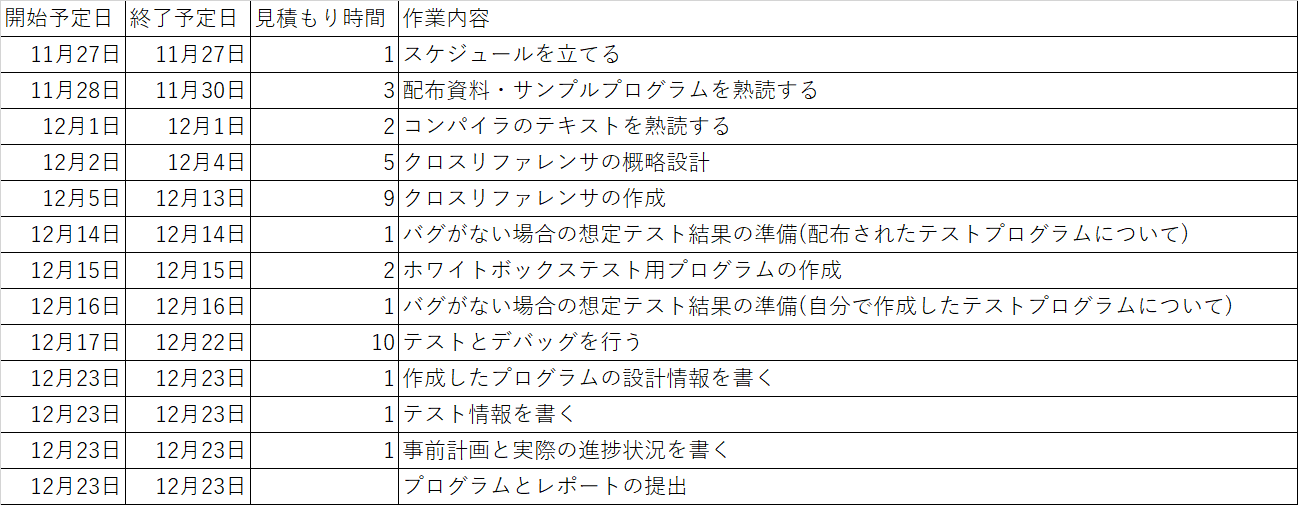
\includegraphics[scale=0.6]{kadai3-jizen.png}
\end{center}
\end{table}

しかし、演習中に計画を以下の表\ref{tb:shusei}のように修正した。
\begin{table}[H]
\begin{center}
\caption{課題3における修正後のスケジュール}
\label{tb:shusei}
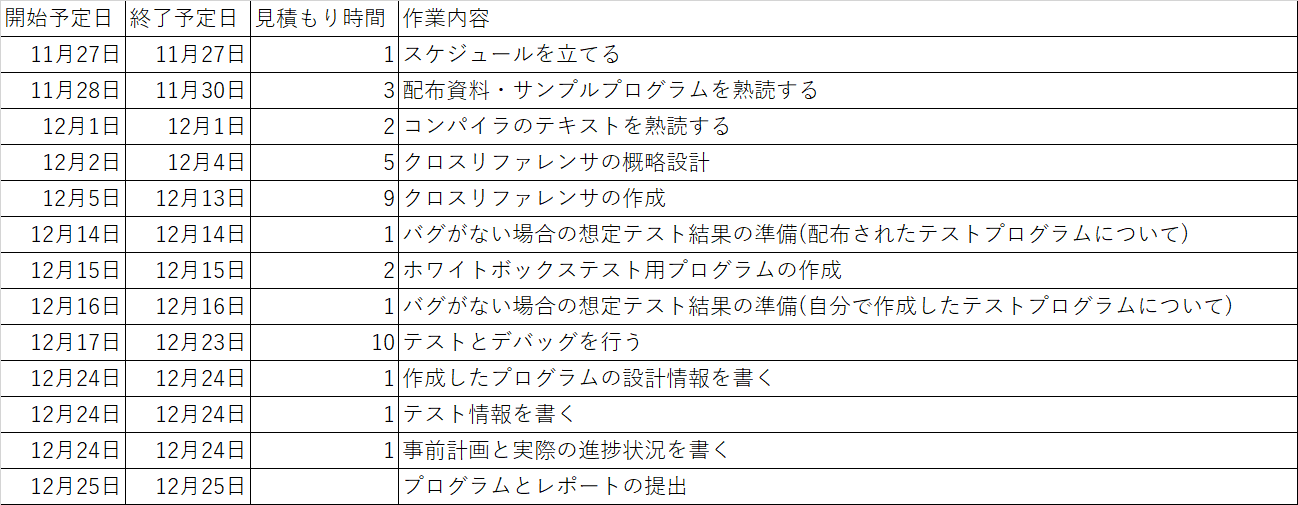
\includegraphics[scale=0.6]{kadai3-shusei.png}
\end{center}
\end{table}
\subsection{事前計画の立て方についての前課題からの改善点}
クロスリファレンサのコーディングとテスト・デバッグの時間を長めに確保した。
\subsection{実際の進捗状況}
表\ref{tb:shusei}のように変更したように、コーディング、テストとデバッグが予想以上に時間がかかってしまった。その他の作業については
だいたい計画通りに進んだ。
\subsection{当初の事前計画と実際の進捗との差の原因}
私自身の理解不足、命令を網羅するために必要なテストプログラムの数の見積もりが少なかったことが原因であると考えられる。
\end{document}
